\thispagestyle{empty}
% Preencher informações em http://ficha.bu.ufsc.br/
% Informações de como preencher em http://portal.bu.ufsc.br/servicos/ficha-de-identificacao-da-obra/
% Salvar preferencialmente em formato pdf
% Talvez seja necessário cortar parte do arquivo
\mbox{}
\vfill
\begin{center}
%  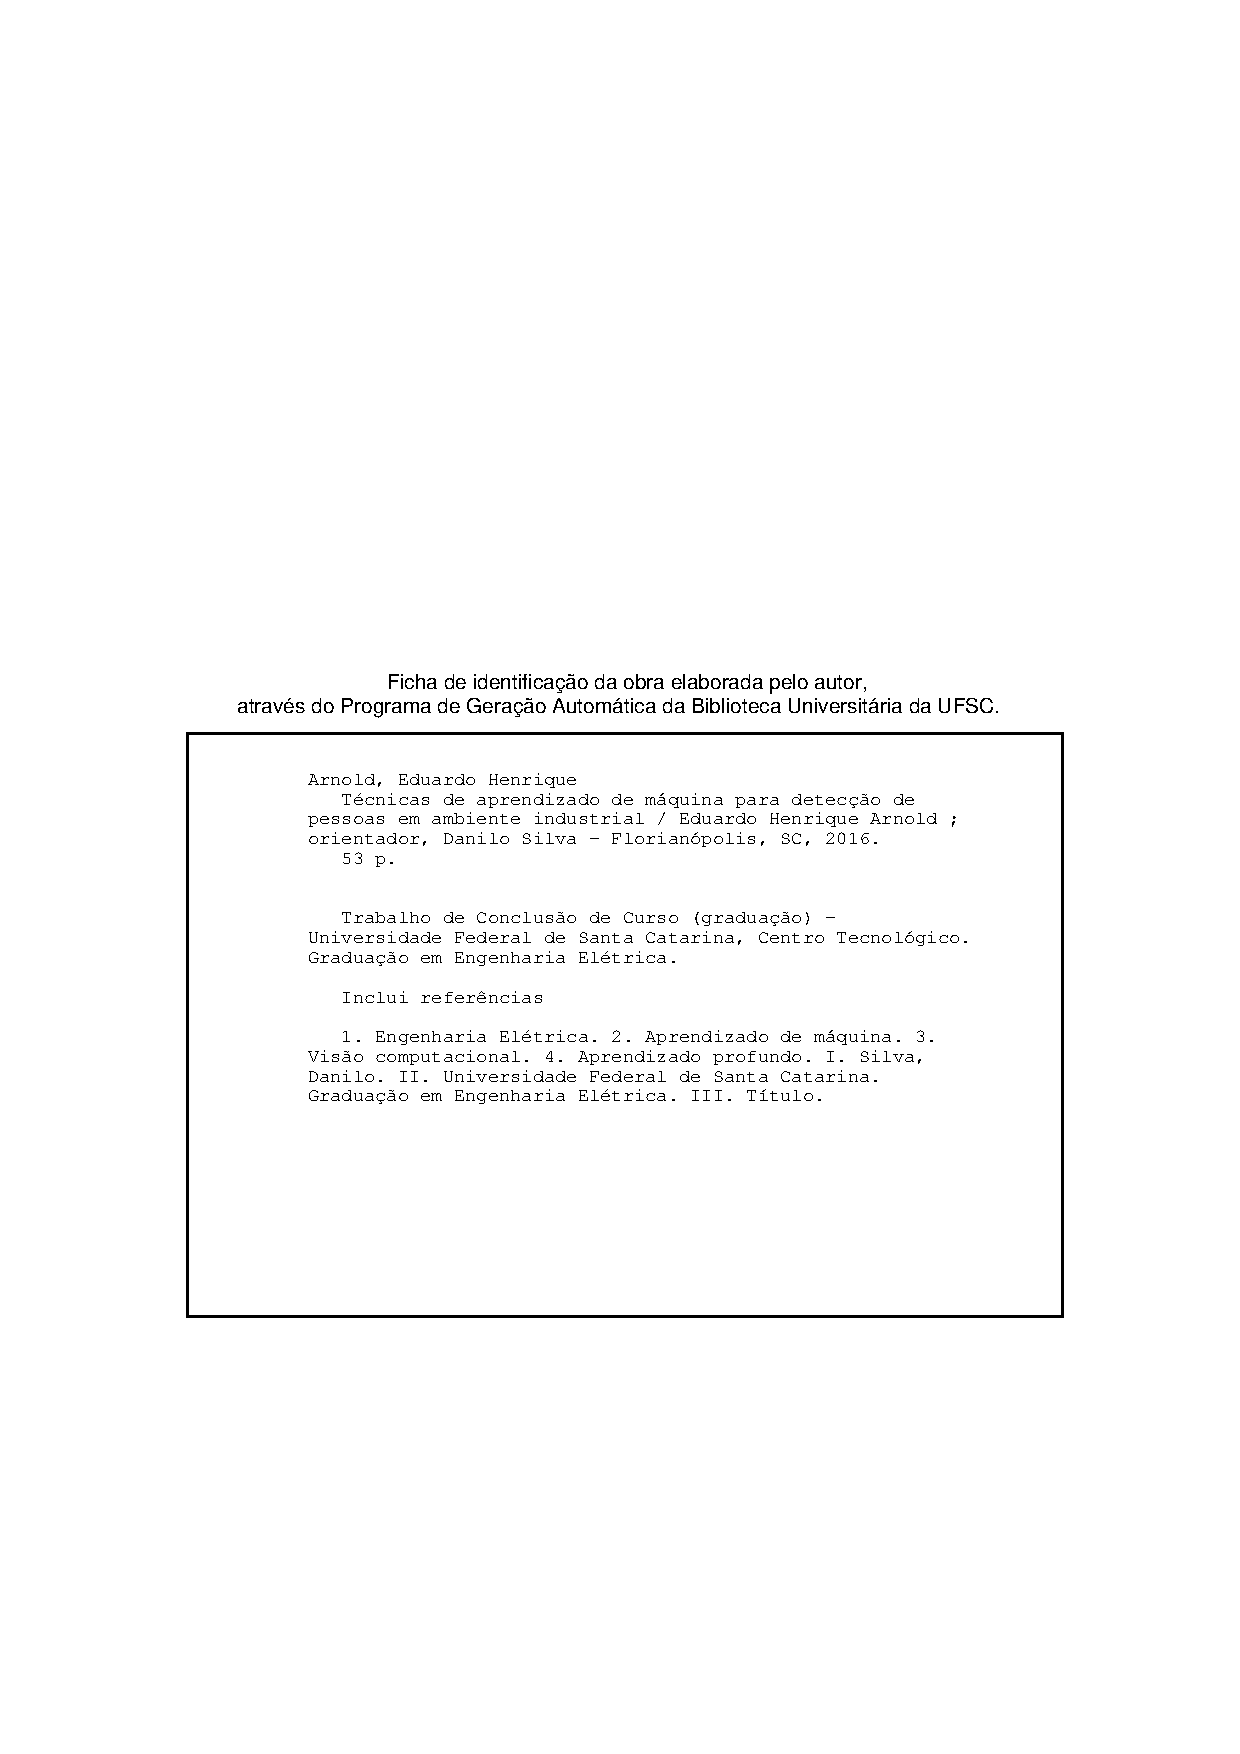
\includegraphics[width=\textwidth]{Ficha_Catalografica}
% Descomentar linha acima para incluir o pdf(png) da ficha catalográfica. Talvez seja necessário alguns ajustes na figura.

% Comentar a partir daqui
Ficha de identificação da obra elaborada pelo autor
através do Programa de Geração Automática da Biblioteca Universitária da UFSC.
\fbox{
\parbox[c][0.4\textheight][c]{\textwidth}{A ficha de identificação é elaborada pelo próprio autor
	
Maiores informações em:

http://portalbu.ufsc.br/ficha
}}
% Comentar até aqui.	
\end{center}
\vfill
\mbox{}

\cleardoublepageempty
